\documentclass[11pt]{article}

\usepackage{sectsty}

% Margins
\topmargin=-0.45in
\evensidemargin=0in
\oddsidemargin=0in
\textwidth=6.5in
\textheight=9.0in
\headsep=0.25in

\title{Interactive Visualization}
\author{Joseph Weibel}
\date{\today}

\setcounter{secnumdepth}{-\maxdimen} % remove section numbering

\usepackage{caption}
\captionsetup[figure]{font=tiny}

\usepackage{wrapfig}
\usepackage{graphicx}
\makeatletter
\def\maxwidth{\ifdim\Gin@nat@width>\linewidth\linewidth\else\Gin@nat@width\fi}
\def\maxheight{\ifdim\Gin@nat@height>\textheight\textheight\else\Gin@nat@height\fi}
\makeatother
% Scale images if necessary, so that they will not overflow the page
% margins by default, and it is still possible to overwrite the defaults
% using explicit options in \includegraphics[width, height, ...]{}
\setkeys{Gin}{width=\maxwidth,height=\maxheight,keepaspectratio}
% Set default figure placement to htbp
\makeatletter
\def\fps@figure{htbp}
\makeatother

\usepackage{apacite}

\usepackage{fancyhdr}
\pagestyle{fancy}
\fancyfoot[L]{Joseph Weibel}
\fancyfoot[R]{Interactive Visualization}

\begin{document}
\begin{titlepage}
    \begin{center}
        \vspace*{0.4cm}

        \Huge
        \textbf{Interactive Visualization}

        \vspace{0.3cm}
        \LARGE
        Report

        \vspace{0.8cm}

        \textbf{Joseph Weibel}

        \vfill

        % TODO image

        \vfill

        \vspace{0.3cm}

        \Large
        FHNW\\
        Data Science\\
        June 2022

        \vspace{1.0cm}

        \normalsize
        Github Repository: https://github.com/josefweibel/ds-ivi-report

        \vspace{0.8cm}

    \end{center}
\end{titlepage}
\pagebreak

\tableofcontents
\pagebreak

Visualisations are a great way to explore data and underpin statements with facts. While static ones are suitable for most cases, interactive plots allow showing more information in the space and allow the viewer to explore the data on their own. These plots can show additional information when the user moves their cursor over one of the data points, or they allow the users to compile their graphics as they like. However, creating such interactive visualisations requires detailed understanding to achieve good usability and avoid confusing the viewers. The following pages will outline theoretical aspects along with practical experience gathered while creating two dashboards created for project works in my studies. One visualises different measurements of a solar energy plant to inspect and compare these. While this is rather technical, the other one shows insights after exploring and comparing data of dementia patients with non-dementia people ~\cite{alzheimers_disease_neuroimaging_initiative_adni_2022}.

\section{Performance}

Interactive visualisations tend to show more attributes and observations than static ones, which increases the risk of performance issues. Moreover, since users can influence its rendering, they need to be rerendered mostly after each interaction. On the other hand, static plots will be rendered once only when they are created. Then, when users want to see them, only a stored file must be shown to them, which computers nowadays can do in a few milliseconds.

The more data to show, the more likely it is that the visualisation suffers under long waiting times and thus the chance that viewers lose interest in the graphic. Especially if viewers need to wait after every interaction, the visualisation can be described as unusable. However, the actual latency is very likely to vary from computer to computer since it depends on the computing power and thus on the computer's hardware. Therefore it is difficult to say from how many data points and features performance issues may arise. Furthermore, performance issues may arise in different parts of creating a plot.

\begin{figure}
    \centering
    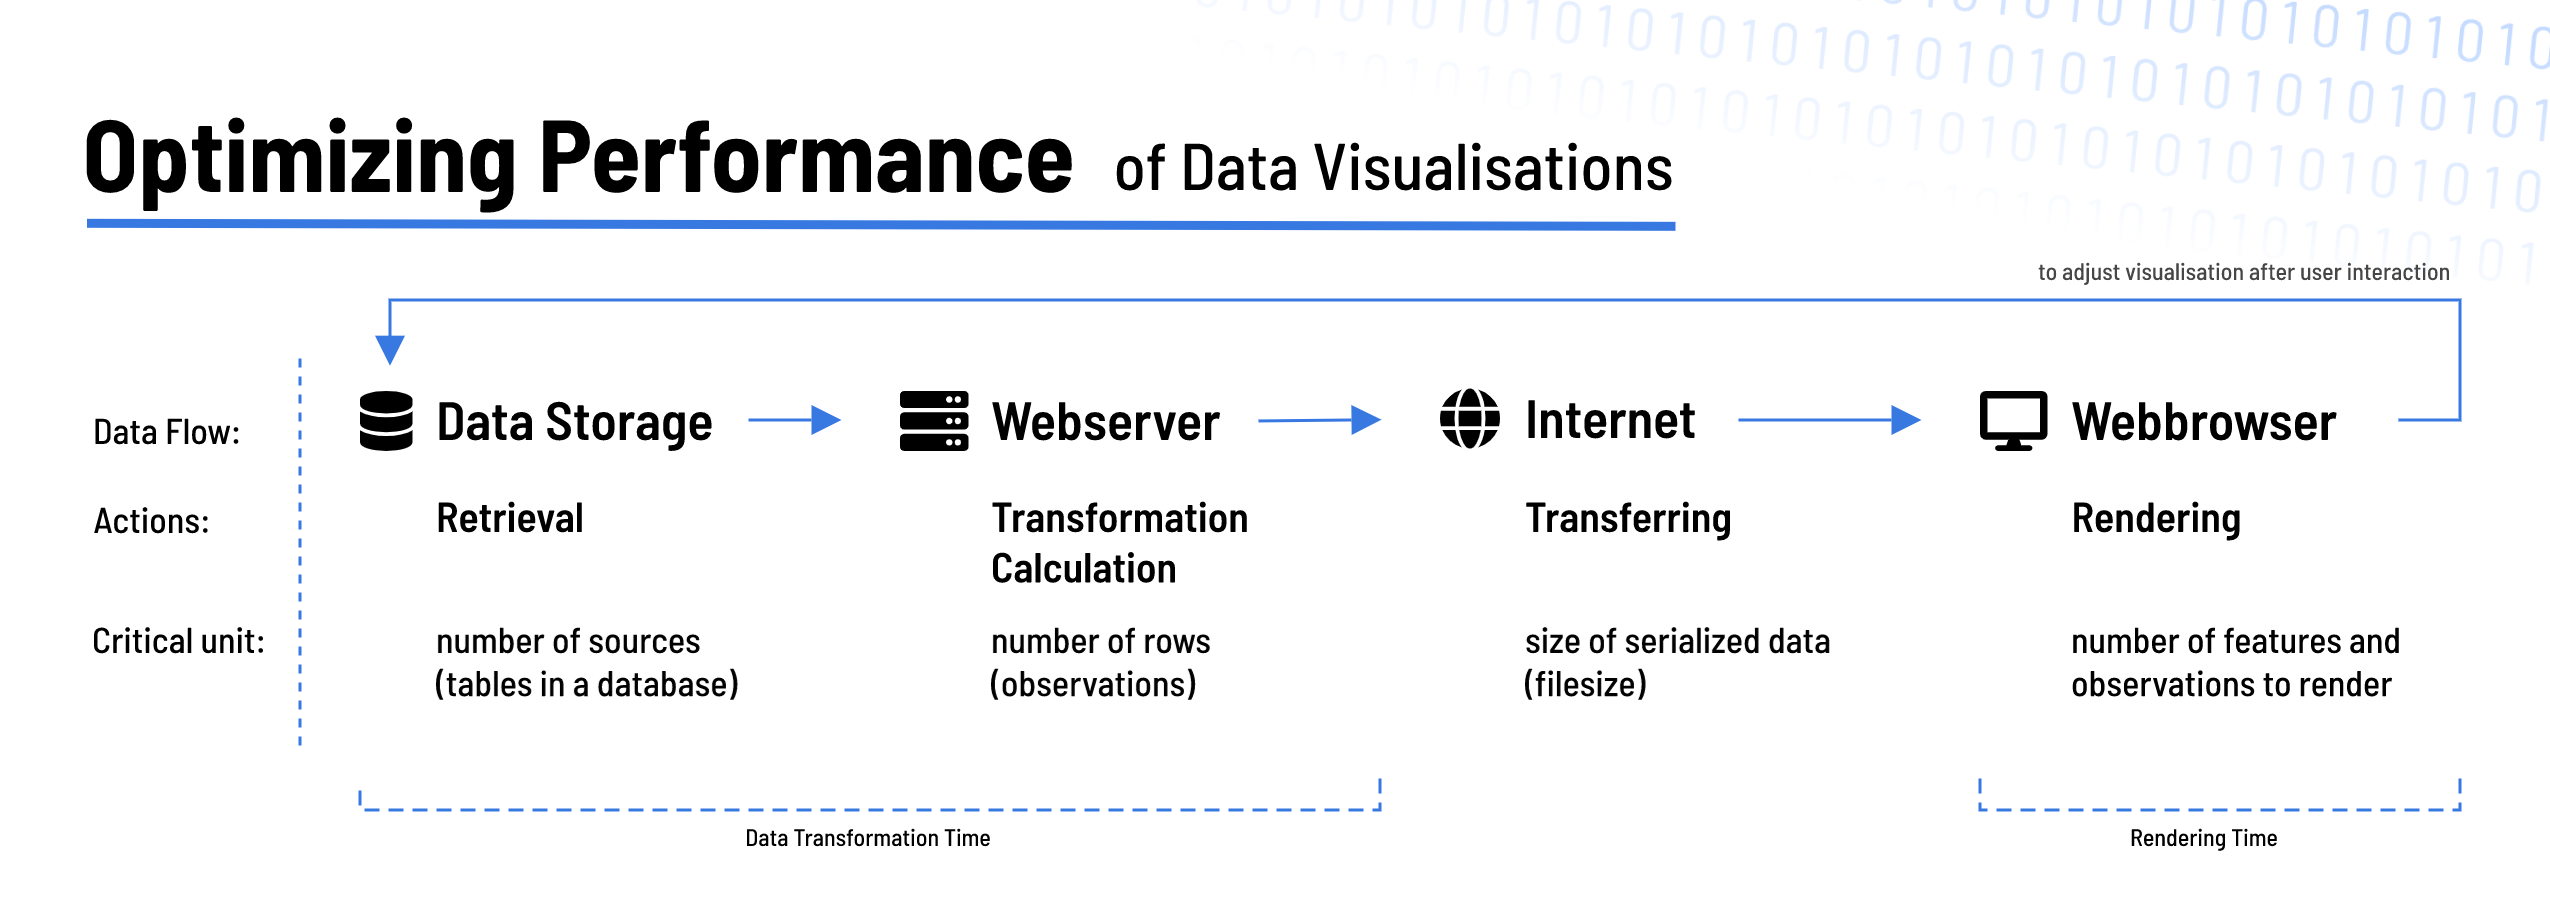
\includegraphics[width=0.7\textwidth]{./performance.png}
    \caption{Infographic showing process to build an interactive visualisation using web technologies. (own graphic)}
\end{figure}

\textit{Figure 1} visualises the four rough parts involved in interactive visualisations built with web technologies. In general, the more data, the more problematic, but the number of sources has a higher impact on data storage systems like databases than the number of features and rows. For example, to transfer data from the webserver to the web browser, only the filesize and the number of requests sent to the server matter. So it is irrelevant if the data consists of a vast amount of rows or attributes. More features affect the web browser's speed slightly more than the webserver since the browser has to add a separate component to the visualisation for every additional feature. Important to know that many web visualisation tools trigger the whole process after most human interactions with the plots.

\subsection{Measurements}

The performance of a visualisation can be quantified by using one of many possible metrics. It is either possible to measure specific overall timeframes or go a step further and use instrumentation to measure individual code blocks ~\cite{isaacs_state_2014}. In web development, a tool called \textit{Lighthouse}~\cite{google_lighthouse_2021} has become the way to measure the performance of websites. It can also be applied to pages containing interactive visualisations and measures specific times like the number of seconds until the user can interact with the site (\textit{Time to Interactive}) or to the point when the first pixel is drawn on it (\textit{First Contentful Paint}).

\begin{wrapfigure}{R}{0.3\textwidth}
    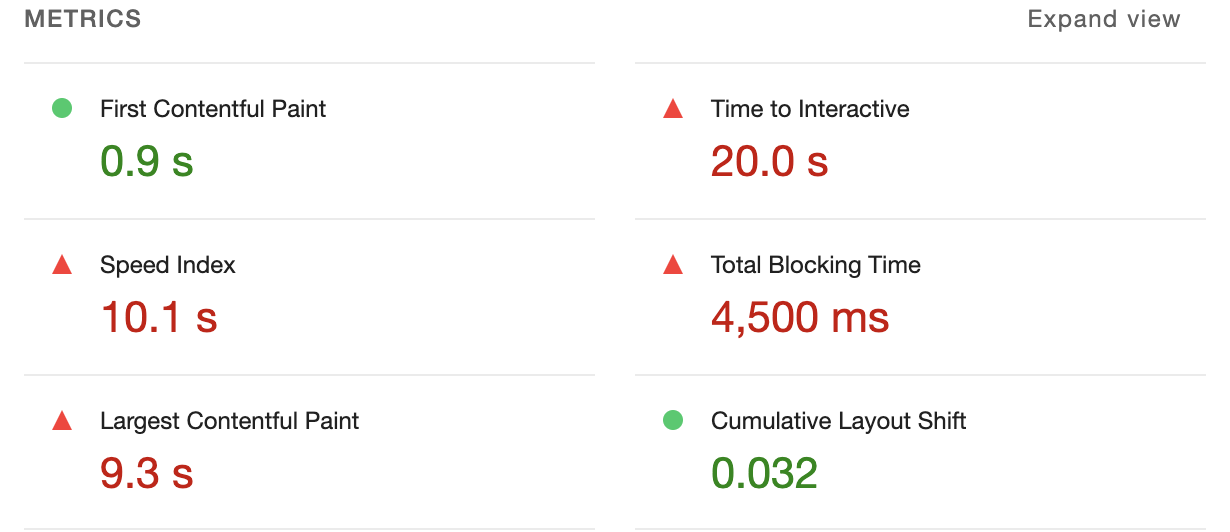
\includegraphics[width=0.3\textwidth]{./lighthouse-1.png}
    \caption{Lighthouse report for dashboard with all observations visible.}
\end{wrapfigure}

The dashboard for the solar energy plant's data suffered severe performance issues. It took quite some time until it got loaded and usable, but each time users changed one of the filters, they had to wait several seconds again for the updated plot. The Lighthouse report (see \textit{Figure 2}) confirms this impression. The total blocking time indicating the cumulated time the user had to wait until the page has been rendered completely is at 4.5 seconds, and the plots have been ready only after 20 seconds. This is too long for a tool to quickly get insights into the data.

\subsection{Solutions}

The possible solutions for slow visualisations are diverse and depend heavily on the problem. If the creation of a plot is deferred because of heavy computations or complex rendering, then outsourcing these tasks to the \textbf{Graphics Processing Unit (GPU)} can speed them up significantly. However, these improvements depend heavily on the available hardware, which is predominantly out of control for data scientists regarding the viewers' machines. For complex visualisations on websites, technologies like \textit{WebGL} should be used, which makes use of the GPU~\cite{mozilla_webgl_2022}.

When showing interactive maps, a technique called \textbf{Tiling} is often used to divide the enormous map into small images to be able to load only the images which are currently in the viewport and required for the current zoom level. This strategy can also be used for other visualisations. For the ones on websites, a library called \textit{Leaflet} is available ~\cite{noauthor_leaflet_2022}.

When calculations after user interactions are not too complex, another improvement is avoiding server roundtrips and recalculating directly in the web browser. However, this is not always possible, primarily when a high-level framework like \textit{Dash} is used. If these can not be bypassed, it is advisable to check for data that can be \textbf{cached}. For example, the ADNI dashboard reloaded the source data on every filter change, which delayed the response by some seconds. However, since the data does not change, it could only be loaded once, and the delay could be removed.

\begin{wrapfigure}{R}{0.3\textwidth}
    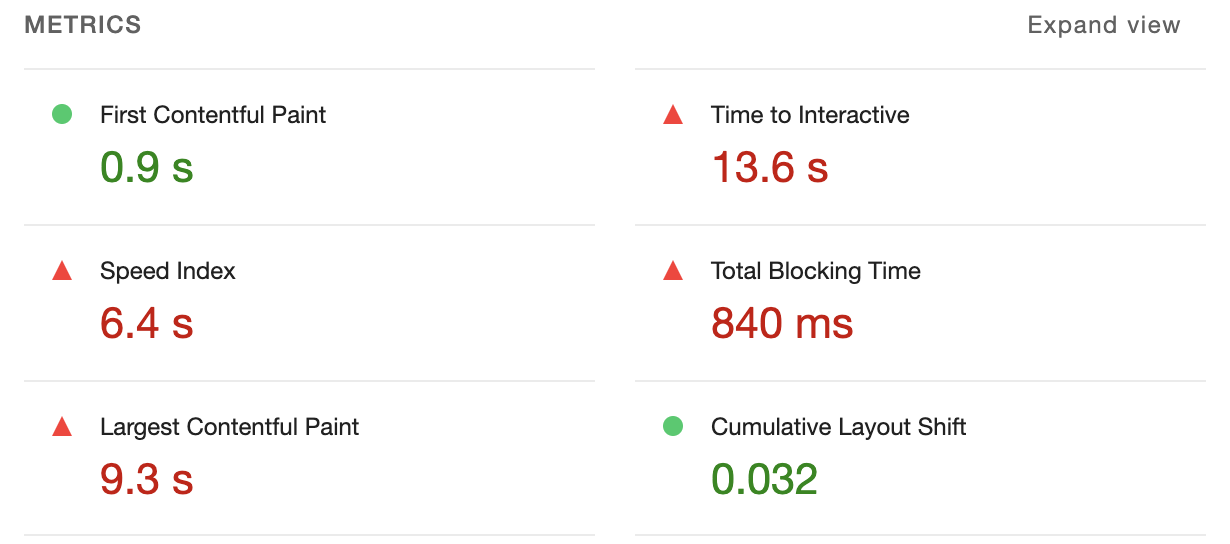
\includegraphics[width=0.3\textwidth]{./lighthouse-2.png}
    \caption{Lighthouse report for dashboard with only observations of one month visible.}
\end{wrapfigure}

Loading data only for one month instead of the complete dataset, which consists of 84'212 observations and 274 attributes, could improve the speed of the energy dashboard. This seemed like a good solution since that much data is overwhelming for the user anyway. Viewers can now switch between months using a filter. Such \textbf{filters} and reducing the \textbf{level of detail} are other practical approaches to improve performance. Certain features could be only shown after the user zoomed into the plot or clicked on specific elements in the plot. If the performance can not be improved anymore and the graphic is still not shown immediately, there should be at least an indicator while the visualisation is rendered. This can be a \textbf{spinner animation} along with a describing text.

\pagebreak
\section{Dashboard Design Principles}

Dashboards are a convenient way to present data by allowing the viewer to customise the charts to get the information they want. To explore realtime data, dashboards are often used. They are also useful for familiarising oneself with a new dataset. However, because these dashboards often visualise many attributes, they can become too complex and overwhelming for the user. Therefore, it is important to follow some principles when creating a dashboard, and depending on the target audience, use case and data, the features and structure will vary greatly. However, the guidelines for static visualisations also apply to interactive visualisations.

\subsection{Shneiderman's Mantra}

A simple strategy for designing a data retrieval tool is Shneiderman's mantra. These three steps provide the user with a structured way to retrieve the information they seek for.

\begin{quote}
    Overview first, zoom and filter, then details-on-demand ~\cite{shneiderman_thousand-fold_1997}
\end{quote}

In order not to overwhelm the user with the vast amount of the entire dataset, them should be presented an \textbf{overview first}. Only the most relevant attributes of the data points should be displayed ~\cite{shneiderman_eyes_1996}. Especially those that answer the user's primary research question. With this first impression, the user is able to understand the most important characterisitics of the data and can now proceed step by step to find the information they are looking for.

After obtaining an overview, the viewer may want to examine certain parts of the data in more detail. By using \textbf{zoom and filter}, it is possible to focus on specific data points and hide irrelevant ones ~\cite{shneiderman_eyes_1996}. Zooming can be done by selecting the desired data directly, or by clicking or scrolling to the area with the data of interest. It should also be possible to use dedicated controls such as buttons to zoom in and out. However, this way of reducing the data only works if the points in the plot are next to each other. In a scatter plot or line chart, it is possible to select the points according to the x- and y-axis by zooming. 

For all other attributes filtering is required for which controls must be available with which the user can make restrictions. The type of controls should be chosen depending on the data type of the attribute to be filtered. A quantitative variable can be limited by a range slider, while dropdowns should be used for qualitative variables. Depending on the meaning of the variable, multiple values should or should not be selectable for the latter. The interface can support the user by indicating the number of remaining results when a certain filter is set. This can be accomplished, for example, by showing the number next to the value in the dropdown or by rendering a small histogram next to a slider showing the distribution of values. Filtering can also mean that complete curves are hidden from the plot. For example, a line chart with several lines can be filtered by removing all but the desired lines. These approaches can reduce the clutter of a visualisation.

Once the user has finally found the points, they can retrieve their \textbf{details-on-demand}. By hovering over or clicking on the data points searched for, the exact values including additional attributes are displayed ~\cite{shneiderman_thousand-fold_1997}. If possible, the filtered and zoomed overview should remain visible in the background so that the user can return and continue with their research without having to adjust the parameters again ~\cite{shneiderman_eyes_1996}. 

In general, a well-usable dashboard records the history of the user's actions and allows the user to undo the last action and also to redo undone actions ~\cite{shneiderman_eyes_1996}. Since dashboards are usually read-only, it would be desirable to have an export function to save the selected data points to a file (e.g. CSV). This file can then be read into a data analysis tool where further evaluations can be undertaken. Furthermore, to avoid the user having to reconfigure zoom levels and filters every time they use the dashboard, it is also helpful if these parameters can be saved in the dashboard.

\subsection{Connecting Plots}

Dashboards with multiple plots based on the same data are not uncommon. Different types of charts can highlight different anomalies in the data, and displaying attributes in different plots keeps them lucid. These related plots should be connected to support the viewer understand the dataset. The connection can be made by linking and brushing the data points in them.

\textbf{Brushing} refers to zooming and filtering the data points. If the number of data points in reduced in one visualisation, the same reduction should be applied to all other visualisations ~\cite{becker_brushing_1987}. If the user zooms into the plot, the same excerpt should become visible on the connected plots, and if the user changes the filter criteria, they should be propagated as well. 

Showing the connection of the same data point in different visualisations is called \textbf{linking} ~\cite{noauthor_linking_nodate}. This can be achieved by highlighting the same data points when one of them is clicked or hovered over by the cursor. This visualises the connection and facilitates the user to rediscover the same data. 

\begin{wrapfigure}{R}{0.2\textwidth}
    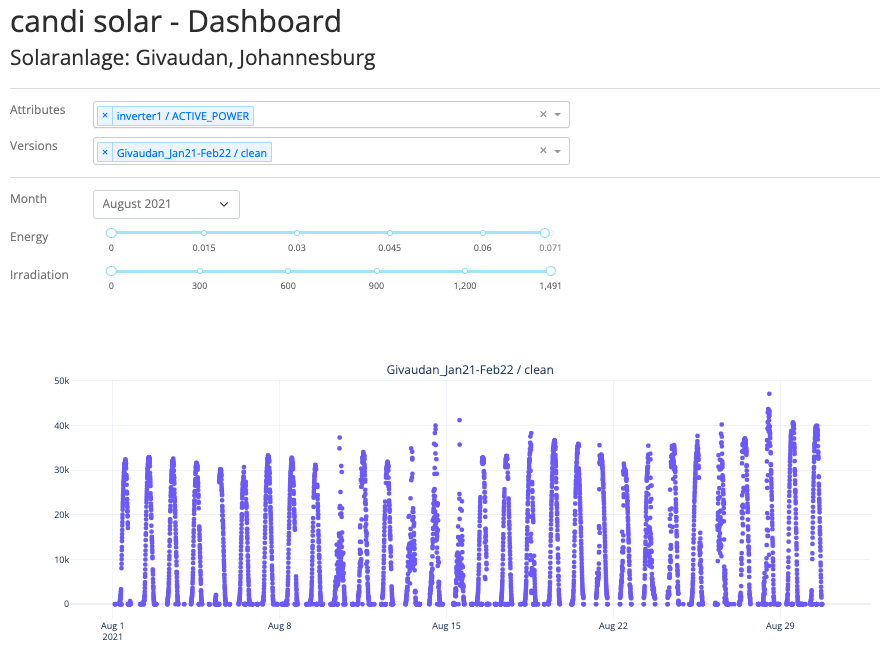
\includegraphics[width=0.2\textwidth]{./dashboard.png}
    \caption{Initial view of dashboard.}
    \label{dashboard}
\end{wrapfigure}

\subsection{Dashboard Example}

To demonstrate these principles, the dashboard with the solar power plant data is used (see Figure \ref{dashboard}). The goal of it is to allow the viewer inspecting the variables that are of interest for them. Therefore, they must first select them from the dropdown at the top of the dashboard. Afterwards, the dashboard shows the values over time in a line chart with a line for each selected variable. There, the user can get an overview of the data for the current month. 

\begin{wrapfigure}{R}{0.2\textwidth}
    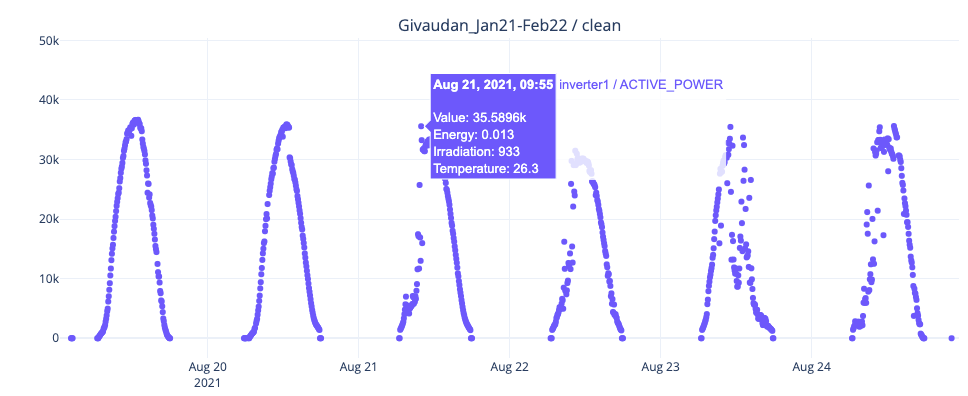
\includegraphics[width=0.2\textwidth]{./dashboard-details.png}
    \caption{Dashboard showing details-on-demand.}
    \label{dashboard-details}
\end{wrapfigure}

Zooming is possible by selecting the desired area by pressing and moving the cursor directly in the plot. The visualisation can be reset to the complete data by double-clicking on it. Lines can be temporarily hidden from the dashboard by clicking on the corresponding attribute name on the right-hand side, or only a specific attribute can be displayed by double-clicking on its name. The data can also be filtered by variables not shown in the plot. Sliders can be used to narrow the range of desired values for energy and irradiation. 

\begin{wrapfigure}{R}{0.2\textwidth}
    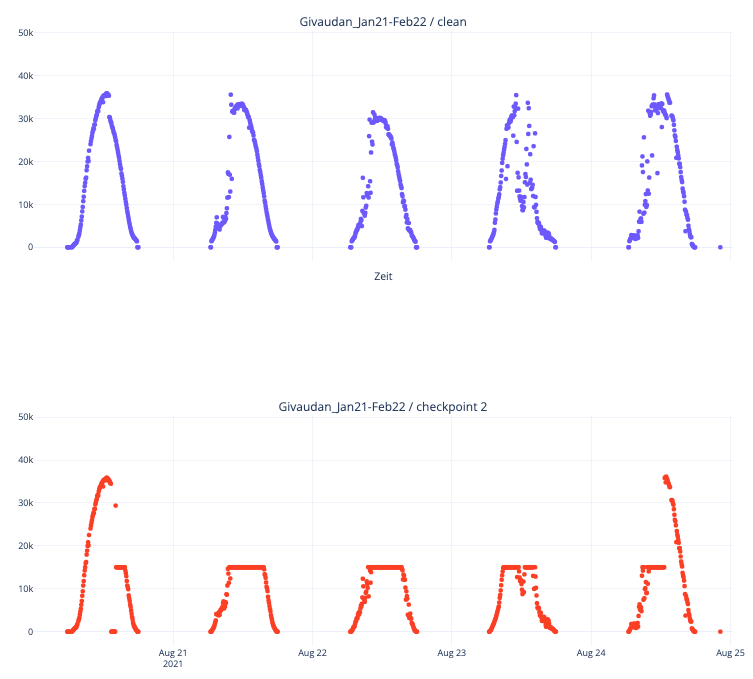
\includegraphics[width=0.2\textwidth]{./dashboard-brushing.png}
    \caption{Dashboard applying principle of brushing.}
    \label{dashboard-brushing}
\end{wrapfigure}

The details of a particular data point can be obtained by pointing the cursor over it. A box will be rendered with the timestamp and the exact values of it. Additional attributes such as energy, irradiation and temperature are also displayed in this tooltip. An example is shown in Figure \ref{dashboard-details}.

This dashboard also supports the comparison of the data after the various cleansing steps to validate the changes. The user can choose the versions of the data they want to compare and a new plot is created for each selected version. As the data come from the same source, they are connected and brushing is applied to the plots. The automatically aligned axes after zooming into the data can be seen in Figure \ref{dashboard-brushing}. Filters and zoom level is propagated to all of them. However, an improvement for the dashboard would be to visually link the data points. 

This dashboard is used by data scientists to familiarise themselves with the data they have received. Once the domain knowlegde and data understanding has been acquired, the dashboard might lose its relevance. Nevertheless, it is reasonable to apply these principles to a temporary dashboard as well.

\pagebreak
\section{HCI Basics}
Lorem Ipsum

\pagebreak
\section{Evaluation}
Lorem Ipsum

\section{Conclusion}
Lorem Ipsum

\pagebreak
\section{Appendix}
Lorem Ipsum

\pagebreak
\bibliographystyle{apacite}
\bibliography{bibliography}


\end{document}
